\section{Clustering}\label{clustering}
In order to find the hotspot(s) defined in \Cref{hotspot}, we considered different clustering techniques.
This section will describe the concepts of clustering as well as the possible algorithms.
This section is based on \citet{pang2006introduction}.

\subsection{Cluster Analysis}
Cluster analysis is a technique used to group data objects based only on the information the data itself contains.
The requirement for membership in a certain cluster is often vague, as several acceptable clusterings can be made on the same dataset.
An example of this can be seen in \Cref{clusterings}, where the same dataset has been clustered in three radically different ways, even though all three could be regarded as correct, depending on the purpose of the clustering.
The clustering therefore depends on the dataset and its purpose.

\begin{figure}[H]
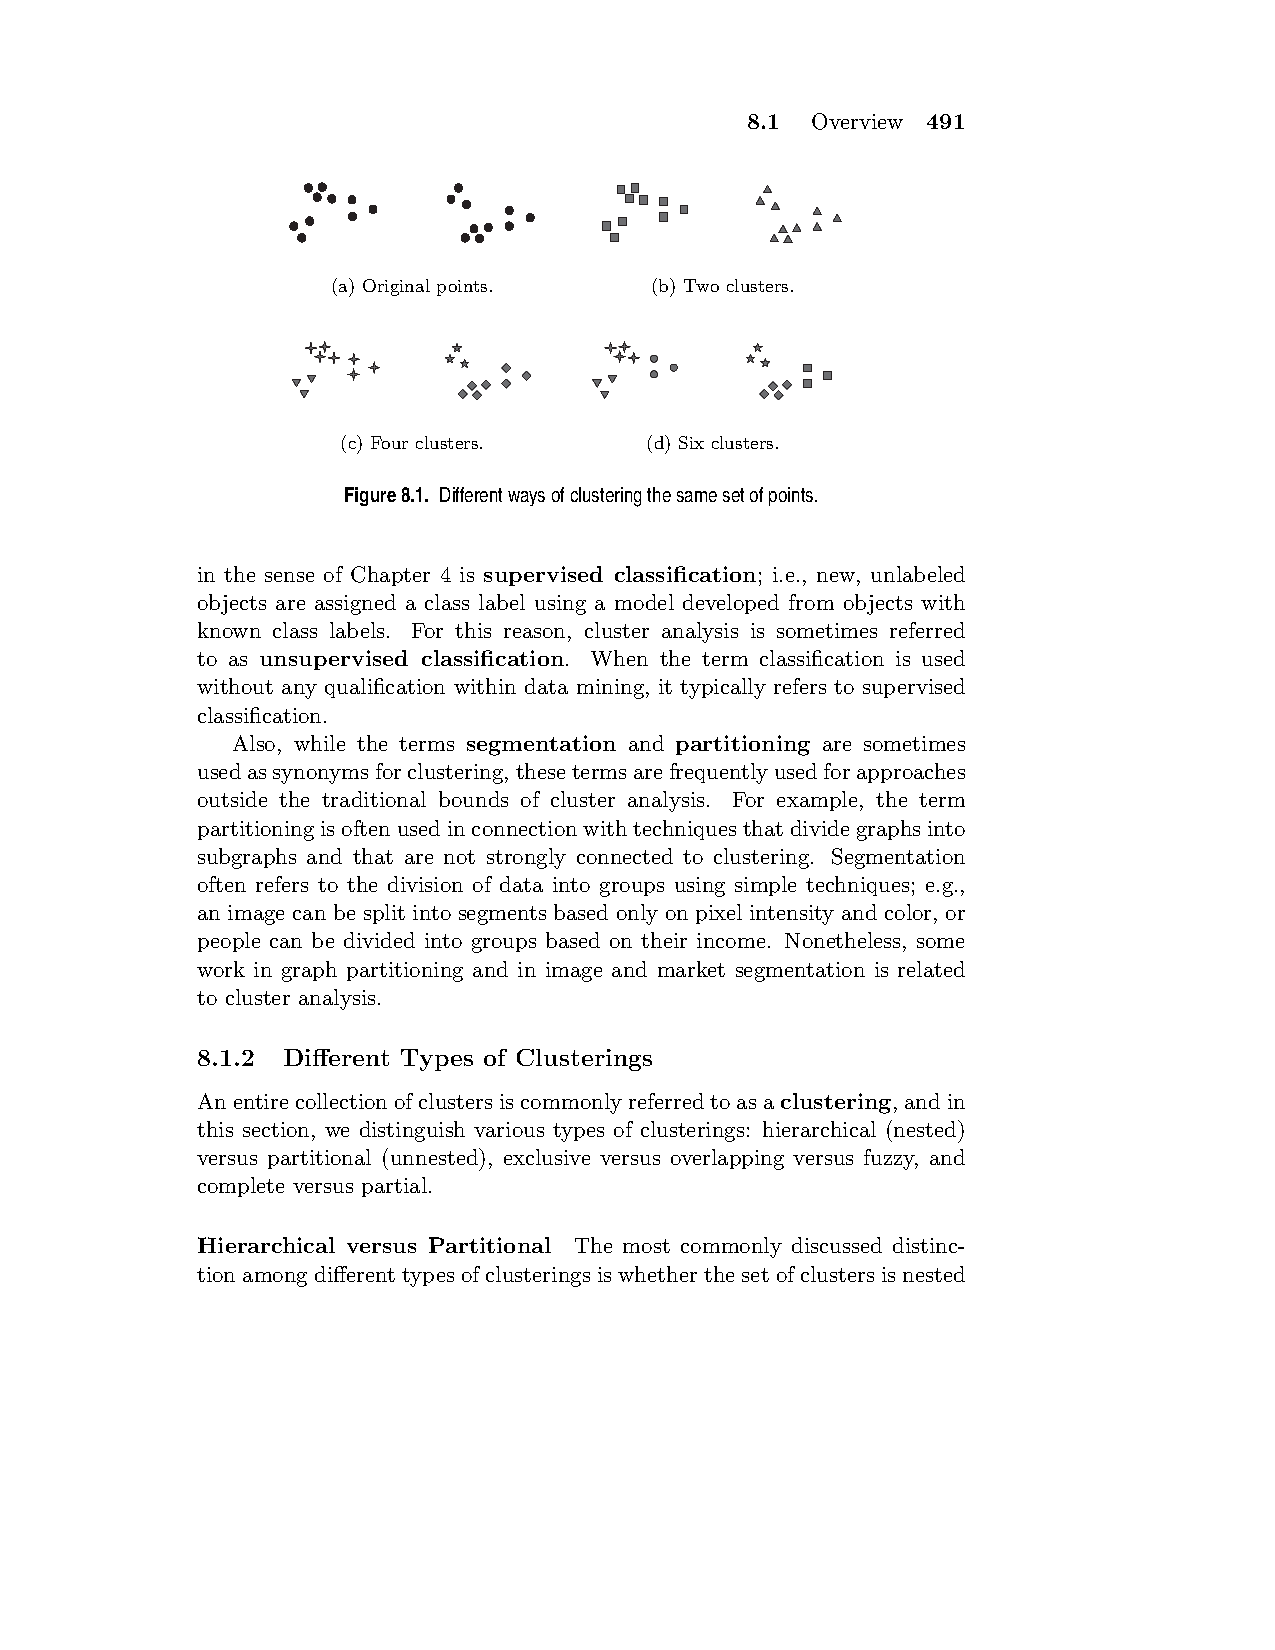
\includegraphics[trim= 3.1cm 19.91cm 5cm 2.5cm, clip=true]{graphics/different_clusters}
\centering
\caption{Different clusterings on the same dataset. From \citet{pang2006introduction}.}
\label{clusterings}
\end{figure}

\subsection{Types of clusterings}

A clustering is a collection of clusters.
This section will introduce the terminology used to describe clusterings. 

\paragraph{Hierarchical versus partitional}
A \textit{partitional clustering} is a division of data into pairwise disjoint subsets, where each object belongs to exactly one subset.
If clusters are allowed to have subclusters, the clustering is said to be \textit{hierarchical}.
A hierarchical clustering is represented as a set of nested clusters organized as a tree, where each node is the union of its children.

\paragraph{Exclusive, overlapping and fuzzy clusterings}

A clustering is \textit{exclusive} if an object is assigned to exactly one cluster.
If an object can belong to more than one group, the clustering is said to be \textit{overlapping}.
If a weight is used to describe the membership of sets, the clustering is said to be \textit{fuzzy}.

\paragraph{Complete versus partial}

A \textit{complete} clustering has every object assigned to a cluster, while a \textit{partial} clustering can have outliers; objects that do not belong to any cluster.

\subsection{Types of clusters}
The purpose of a cluster depends on the kind of data set it is applied on.
In this section, the different notions of a cluster will be presented.

\paragraph{Well separated}
A cluster is a set of objects, where the objects that are similar are grouped in a cluster. 
Sometimes a threshold is used to define a minimum similarity. 
All objects in a cluster need to be at least as similar to all other objects in the cluster, for an object to be in the cluster.

\paragraph{Prototype based}
Objects are placed in clusters based on the prototypes that define the clusters.
An object is placed in the cluster where the object is more similar to the prototype of that cluster, than to the prototype of all other clusters.

These prototypes can be either the average value of a cluster, or the most representative object of a cluster.

\paragraph{Graph based}
If the data can be represented as a graph, with the objects as nodes, clusters can be defined as connected components in the graph.

\paragraph{Density based}
A cluster is defined by the density of the data objects.
A cluster is a dense region surrounded by a low density region.

\subsection{Our data and purpose}
The data we need to cluster is GPS data from the bikes.
\mikael{Som mine tidligere kommentarer, klart defineret begreb. GPS data, i denne kontekst, dækker kun over stillestående punkter.}
We expect the points to be distributed in a wide area, but clustered around places where people place the bikes.
These clusters may have different size, depending on the physical properties of the places the bikes are left.

The purpose of the clustering is to find the areas where the bicycles are being used the most, in order to make predictions on when a bike will arrive in those areas.
\mikael{Bør det ikke benævnes som hotspot her, da vi har defineret hotspots?}

Based on this description we need a hierarchical, exclusive, partial and density based clustering.

Hierarchically, because it makes it easy to locate what cluster a point belongs to by traversing the resulting tree.
\mikael{Er det her ikke forkert, har vi ikke en partitional clustering?}
\stefan{vi har ikke hierarkisk, men ud fra vores data ville det sandsynligvis være det bedste valg, da det er lettere at finde ud af hvilket cluster et punkt er i.
(jeg har omformuleret argumentet en smule siden Mikaels kommentar)}

It needs to be exclusive because we want the clusters to be separated from each other so any point on the map is either in one cluster or not in any cluster.
We want to find out where the bikes spend most of their time and therefore we want a density based partial clustering.

\subsection{Techniques}
This section will explore the techniques that exist in cluster analysis, as well as evaluate them, based on the requirements stated in the previous section.

\subsubsection{K-means}
K-means is a technique that creates a partitioning from prototypes, where the prototypes are the centers of clusters.

The basic algorithm takes a number $K$ and generates $K$ initial center points.
Each data object is then assigned to the nearest center point.
The center points are now updated to be the center of the created clusters.
These steps are repeated until no point changes cluster, or the center points do not change.

Because we do not have a way of finding $K$ before running the algorithm, this approach is not applicable to our problem.

\subsubsection{Hierarchical Clustering}
Hierarchical clustering arranges the points in a hierarchy, dependent on the distance between points.
Hierarchical clustering can be performed either by starting at the top of the tree or at the bottom.
\textit{Agglomerative hierarchical clustering} starts by considering all points as being in individual clusters, then generating the hierarchy by merging the closest clusters.
\textit{Divisive hierarchical clustering} starts by considering all points as being in a single cluster, then continues by splitting the clusters at each step.

We would like our clustering to be hierarchical, but this algorithm does requirement for a density based clustering.
\mikael{Det her siger det stik modsatte af hvad 2.2.4 siger.}
\stefan{jeg har opdateret konklusionen, men jeg ved ikke hvordan vi argumenterer for at density er vigtigere end hierarki}

\subsubsection{DBSCAN}\label{clustering:DBSCAN}
DBSCAN is a density-based clustering algorithm, which locates regions of high density that are separated by regions of low density.

\stefan{der mangler måske et sted hvor der står at DBSCAN er superduper, inden vi begynder at gå i detaljer med den?}

\paragraph{Center based point density}
There exists different methods of determining density in a set of data points.
One approach is to use a point as a center and calculate the number of points that are within a certain radius of the point.
Using this measure it can be determined whether a point is placed in a dense region (a core point), at the edge of a dense region (a border point), or is in a region with sparse density (a noise point).
The exact definition of the three types of points are as follows\cite{pang2006introduction}:

\begin{description}
\item[Core point] These points have at least $ MinPts $ points in a radius of $ eps $ from it.
Here, $ MinPts $ is the minimal number of points in the vicinity of a point, regarded as dense by the user, and $ eps $ is the radius in which to look for these points.

\item[Border points] A point that is not a core point, but is in the neighbourhood of a core point. 
One point can be a border point to several core points.

\item[Noise point] Any point that is neither a core point or a border point. 
\end{description}

\begin{figure}
\fbox{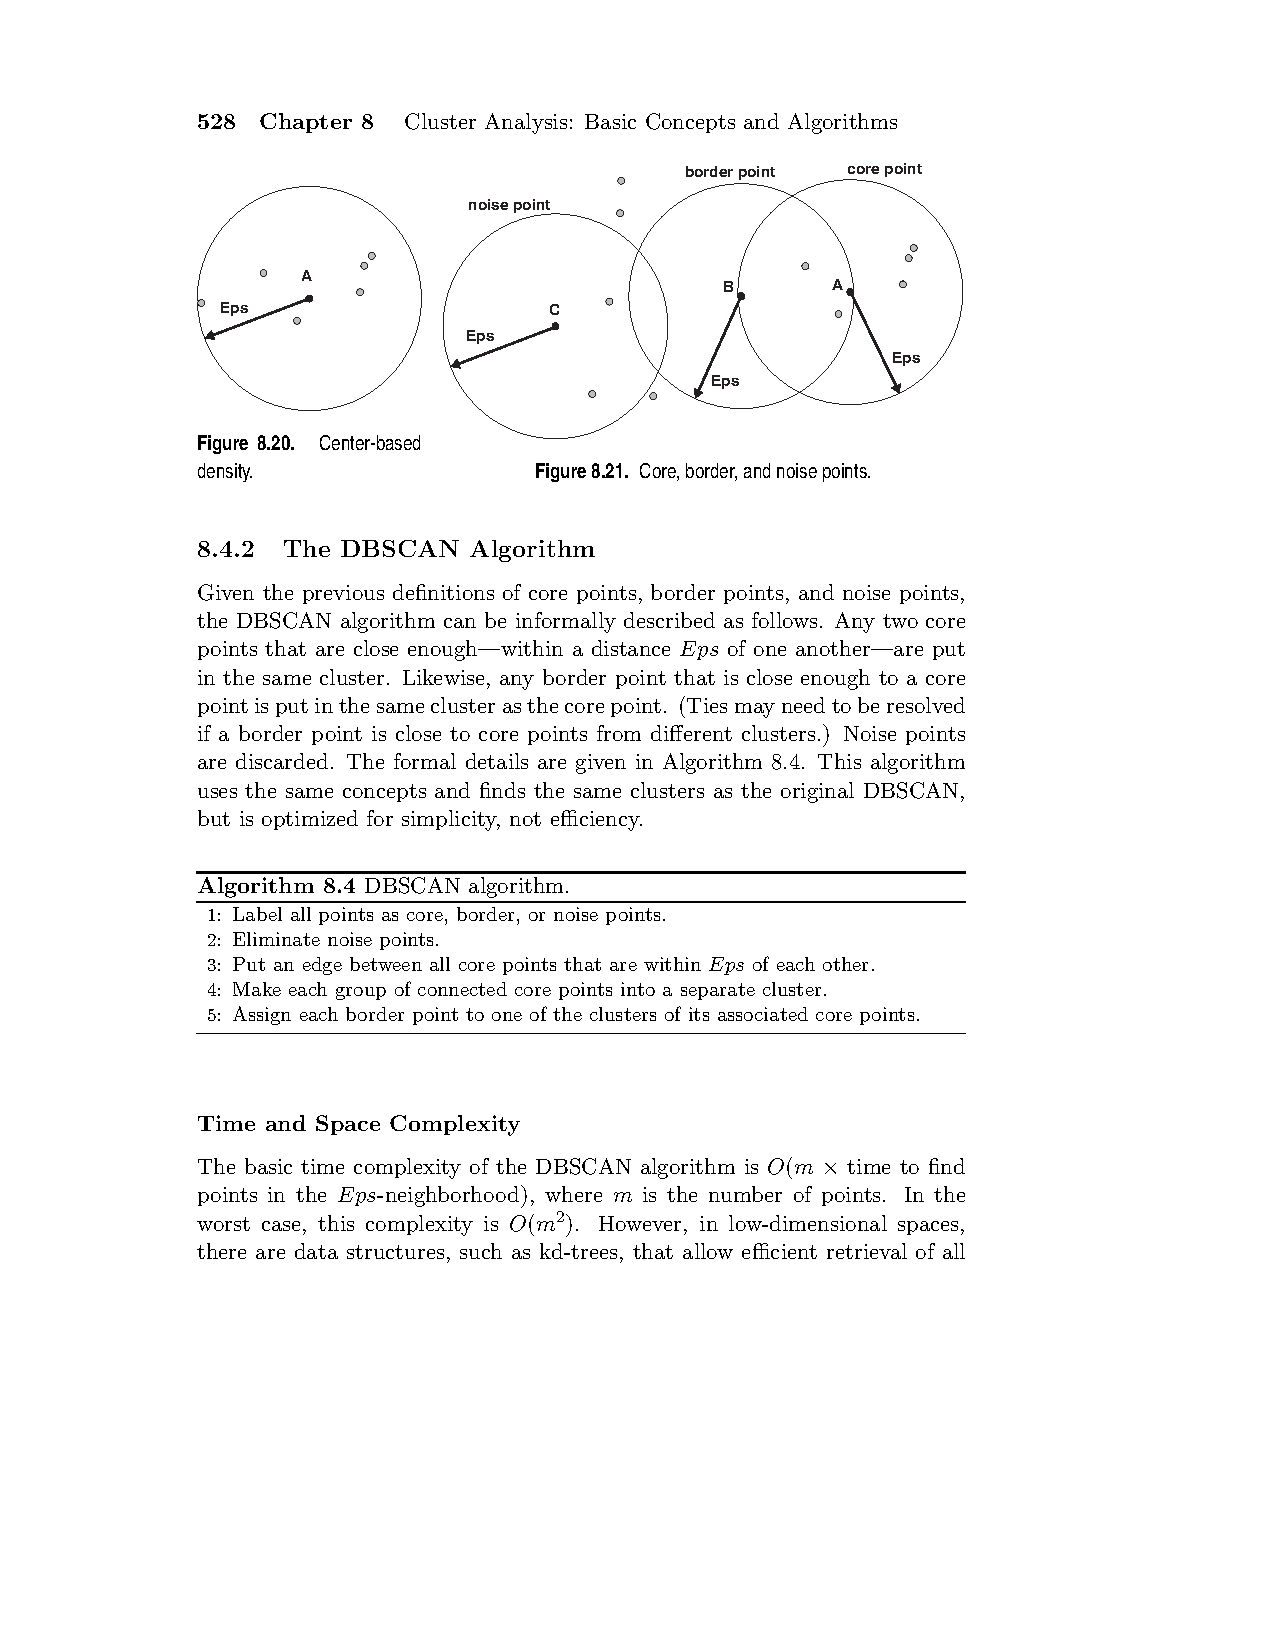
\includegraphics[trim= 3.1cm 20.61cm 5cm 2.5cm, clip=true]{graphics/DBSCAN_point_types}}
\caption{The three types of points in the clustering algorithm DBSCAN. Taken from \cite[page 528]{pang2006introduction}.}
\label{dbscan_point_types}
\end{figure}

A visual description can be seen on \Cref{dbscan_point_types}.
Given these definitions, the algorithm is described in \Cref{dbscan-algo}.

\begin{algorithm}
DBSCAN(D, eps, MinPts)\\
	C = 0\\
	\For {each unvisited point P in dataset D mark P as visited\\}
	{
		NeighborPts = regionQuery(P, eps)\\
		\eIf {sizeof(NeighborPts) < MinPts}{
			mark P as NOISE\\
		}
		{
			C = next cluster\\
			expandCluster(P, NeighborPts, C, eps, MinPts)
		}
	}
\caption{The DBSCAN clustering algorithm}\label{dbscan-algo}
\end{algorithm}

\begin{algorithm}
expandCluster(P, NeighborPts, C, eps, MinPts)\\
	add P to cluster C\\
	\For {each point Pn in NeighborPts\\}
	{
		\If{Pn is not visited\\}
		{
			mark Pn as visited\\
			NeighborPtsn = regionQuery(Pn, eps)\\
		}
		\If {sizeof(NeighborPtsn) >= MinPts\\}
		{
			NeighborPts = $ NeighborPts \cup NeighborPtsn $\\
			\If {Pn is not yet member of any cluster\\}
			{add Pn to cluster C\\}
		}
	}
\end{algorithm}%(Pn) is used instead of (p') in source (wiki).

\begin{algorithm}
regionQuery(P, eps)\\
	\Return {all points within the eps-neighborhood of P (including P)\\}
\end{algorithm}

\subsection{Summary} Of the three presented algorithms, only the DBSCAN algorithm fits our need for an exclusive, partial and density-based clustering algorithm.
We therefore use this algorithm to detect clusters in our data, to be used as the hotspots in our model.
The hierarchical need is covered by saving the clusters in a tree data structure\footnote{This was not implemented, see \Cref{ref:ods}.}.
\mikael{Samme konflikt som tidligere nævnt.}
